\documentclass[../main.tex]{subfiles}
\graphicspath{{\subfix{images/}}}


\begin{document}

\section{Methodology}
\subsection{Watching conspiracy videos}
In order to determine how different watch strategies affect the YouTube algorithm, a python script was
created to automatically log into a Google account and proceed to watch YouTube videos. The script was
made using Selenium WebDriver: a suite of tools used for browser automation. 

In the following sections, each aspect of the initial experiment will be explained. Firstly, an explanation
will be given about how to log into Google accounts using a python bot. Then, the watch strategies as
mentioned in the research question will be defined, followed by a description of their video watching 
behavior. Afterwards, some restrictions about the videos being watched will be mentioned. Additionally the
actual script allowing the bots to be run will be described. Lastly, the precise form of the output of the script will be explained. 

\subsubsection{Google login}
Due to Google's strict policy regarding automation within their ecosystem, many obstacles are put into
place to prevent users from logging into a Google account using automated software such as a selenium 
script. To circumvent this restriction, two steps had to be taken. Firstly, the selenium WebDriver had to
be accompanied by the selenium-stealth package, which removes metadata about the current browser, so that
it is less obvious that a WebDriver is being used. Additionally, because this metadata was removed, the 
Google login service was unable to check what browser the client was using. This results in a warning to 
the user that their current browser may be insecure, which prohibits them from logging in. To avoid this 
warning, the Google account needs to have been created within a WebDriver, such as Google's ChromeDriver 
or Mozilla's GeckoDriver. Therefore, all twenty accounts were manually created in ChromeDriver. Since 
Google accounts require a phone number verification upon creation, six free (prepaid) SIM cards were 
ordered from various providers in order to create the accounts. Each SIM card could create two to three 
accounts before it was blocked due to being used too many times. 

\subsubsection{The watch strategies}
After all accounts had been created, they were subdivided into four distinct watch strategies, making for
a total of five accounts per strategy. 

\begin{description}
\item[1. Random videos (baseline)] The first watch strategy is the simplest one. The bots following 
it will watch random \textit{non-conspiracy} videos from a dataset (for a description of the dataset see \ref{Machine Learning}). This watch strategy is used as the baseline to compare the other three strategies to.

\item[2. Random conspiracies] The second strategy is similar to the first: the adhering bots watch random
\textit{conspiracy} videos from the dataset. 

\item[3. Watch-next recommendations] The penultimate strategy starts off in the same way as strategy 2: it 
chooses a random conspiracy video from a dataset to watch. However, it then watches the four most similar 
videos in the dataset (based on cosine similarity) in order to allow the algorithm to get a feel for the 
user's interests. After watching those five initial videos, it starts looking at the recommended videos 
displayed next to the current video and chooses the recommendation that is most likely to be a conspiracy 
video (out of the first twenty recommendations). These recommendations consist of a combination of 
recommendations based on the content of the current video and the personalized recommendations of the 
user. It is expected that, by using this strategy, bots are likely to go \textit{down the rabbit hole} and eventually 
end up in a filter bubble.

\item[4. Homepage recommendations] Finally, the last strategy is similar to the previous one, though
with one alteration: rather than choosing a recommended conspiracy video from the list of recommendations 
next to the current video, it will choose a recommended video from the YouTube homepage of the account 
(again out of the first twenty recommendations). Compared to the third strategy, this will lead to the user
watching more personalized recommendations rather than content-based recommendations, possibly speeding up 
the creation and/or increasing the strength of the filter bubble.

\end{description}
For strategy 3 and 4, the likelihood of a recommendation being a conspiracy video was estimated by a 
neural network using the title, description, transcript, channel description, and channel keywords of the 
specific video. Though this is more information than a regular user would have to their disposal, it has to 
be kept in mind that humans are able to interpret the thumbnail of the recommendations, can have 
foreknowledge about the channel that is uploading the video or the subject being mentioned in the title, et cetera.
Thus, the choice was made to allow the neural network to consider the transcript and look at general information 
about the uploader to balance the scales. 

Each strategy was executed by five different accounts in order to decrease the probability of a 
random streak of videos altering the result. The individual accounts watched a total of fifteen
videos as described by their watch strategy for a total of three hundred videos watched by the script. 

Additionally, to simulate real-world user behavior, the average watch time for the videos was normally
distributed with a mean of 55\% and a standard deviation of 25\% \citep{park2016data, lang_2018}. The 
watch time was not be able to exceed a value of 100 or subceed a value of 0, as a video cannot be watched 
for more than 100\% or less than 0\%. In the same vein, the clicking behavior of users was simulated as 
accurately as possible. Whenever none of the recommendations were predicted to be conspiracy videos, the 
probability of a user clicking on a video at position $k$ within a given list of recommendations (its 
click-through rate: $CTR$), was determined using the following formula:

\begin{equation}
CTR(k; N, \alpha) = \frac{1/k^\alpha}{\sum_{n=1}^{N} (1/n^\alpha)}
\end{equation}

Wherein $N$ is the total number of recommendations and $\alpha$ is the distribution's exponent value 
($\alpha = 0.78$) \citep{zhou2010impact}. Using this formula, when considering the first twenty 
recommendations, the first recommendation will have a click-through rate of approximately 20.6\%, after 
which the CTR quickly decreases, until a probability of 1.9\% at the twentieth recommendation. 

\subsubsection{Running the bots}
After the accounts were logged in, they started watching YouTube videos according to their watch
strategy. However, some restrictions were put into place to make sure running the bots did not take too long, as
three hundred videos had to be watched in total. For example, the bots were not allowed to watch videos over an
hour long, nor were they allowed to watch live streams, as those could theoretically go on infinitely.
Additionally, the random videos at the start of the third and fourth strategy were first manually inspected to make
sure the bots would not start the experiment by watching a falsely flagged conspiracy video. Considering the way in
which the dataset was created (see \ref{Machine Learning}), it is possible that some videos that are flagged as
conspiracy videos are, in reality, normal videos. This could happen whenever a conspiracy channel uploads a regular
video (e.g. a holiday video, promotion of some product, etc.). These \textit{false positives} are far and
few between, however, having one of them be selected as the first video for strategy 3 or 4 had to be prevented, as
that could have greatly altered the final results. With these restrictions in mind, the following script was 
created and run for all twenty bots, keeping track of the videos they watched and the homepage 
recommendations they had after each video:

\vspace{0.25in}

\begin{algorithm}[H]
 \KwData{User information and a video dataset}
 \KwResult{The watched videos and homepage recommendations of the user}
 
 \vspace{0.075in}

 \For{twenty bots}{
    initialize WebDriver\;
    log into Google account\;
    \vspace{0.05in}
    
     \For{fifteen videos}{
      \eIf{there is a recommendation to be watched}{
        go to the link\;
       }{
        pick a random video to watch based on usertype\;
        determine how long it will get watched\;
        go to the link\;
       }
       \vspace{0.05in}
       get video metadata and store for overview of watched videos\;
       watch video for given amount of time\;
       \vspace{0.05in}
       \uIf{usertype == 3}{
        pick recommendation next to current video to watch next\;
        determine watch time for found recommendation\;
       }
       \vspace{0.05in}
       go to YouTube homepage\;
       store current recommendations for overview\;
       \vspace{0.05in}
       \uIf{usertype == 4}{
        pick homepage recommendation to watch next\;
        determine watch time for found recommendation\;
       }
     }
 }
 \vspace{0.05in}
 \textbf{return} watched videos and homepage recommendations\;
 \caption{Watch YouTube videos according to a watch strategy}
\end{algorithm}

\vspace{0.25in}

Running the script for all twenty bots resulted in two different datasets: the first containing
the videos watched by the bots and the second containing the homepage recommendations for all bots, after 
each number of videos watched. To determine the influence of the watch strategies on the algorithm, the 
recommendations were labeled as being either conspiracy or non-conspiracy videos by the classifier. By then 
grouping all recommendations by their watch strategy and the number of videos watched before them (e.g. the 
recommendations after the third video watched by all bots with strategy one), it was possible to calculate 
aggregates about general statistics of the recommendations, such as view count and video duration, and the 
percentage of conspiracy videos present amongst them. This lead to four groups with fifteen entries of 
different statistics (one for each video watched). In order to find out whether any of the differences 
between the groups were significant at any point, a number of independent samples t-tests were performed. 

\subsubsection{Outputs of the experiment}
To create the initial recommendation dataset, the bots stored the following information about their top 
twenty recommendations after each video watched: 
\begin{itemize}
    \item the id of the bot that had gotten the recommendations;
    \item the amount of videos watched before the recommendation was given;
    \item the URL of the video being recommended;
    \item the URL of the channel that uploaded the recommendation.
\end{itemize}
To then allow the classifier to label the videos, and to calculate the aggregates per strategy, additional 
data was gathered using YouTube's API. For each recommendation, the title, description, transcript, 
(dis)likes, views, video duration, channel description, and channel keywords were collected. The title, 
description, transcript, channel description, and channel keywords were collected in order for the 
classifier to label the videos, as will be further explained in section \ref{Machine Learning}. The other 
features were collected in order to calculate the aforementioned aggregates. An example of the output can be seen
in figure \ref{fig:dataframe}.

\begin{figure}[t]
  \textbf{Example DataFrame}\par\medskip
  \centering
  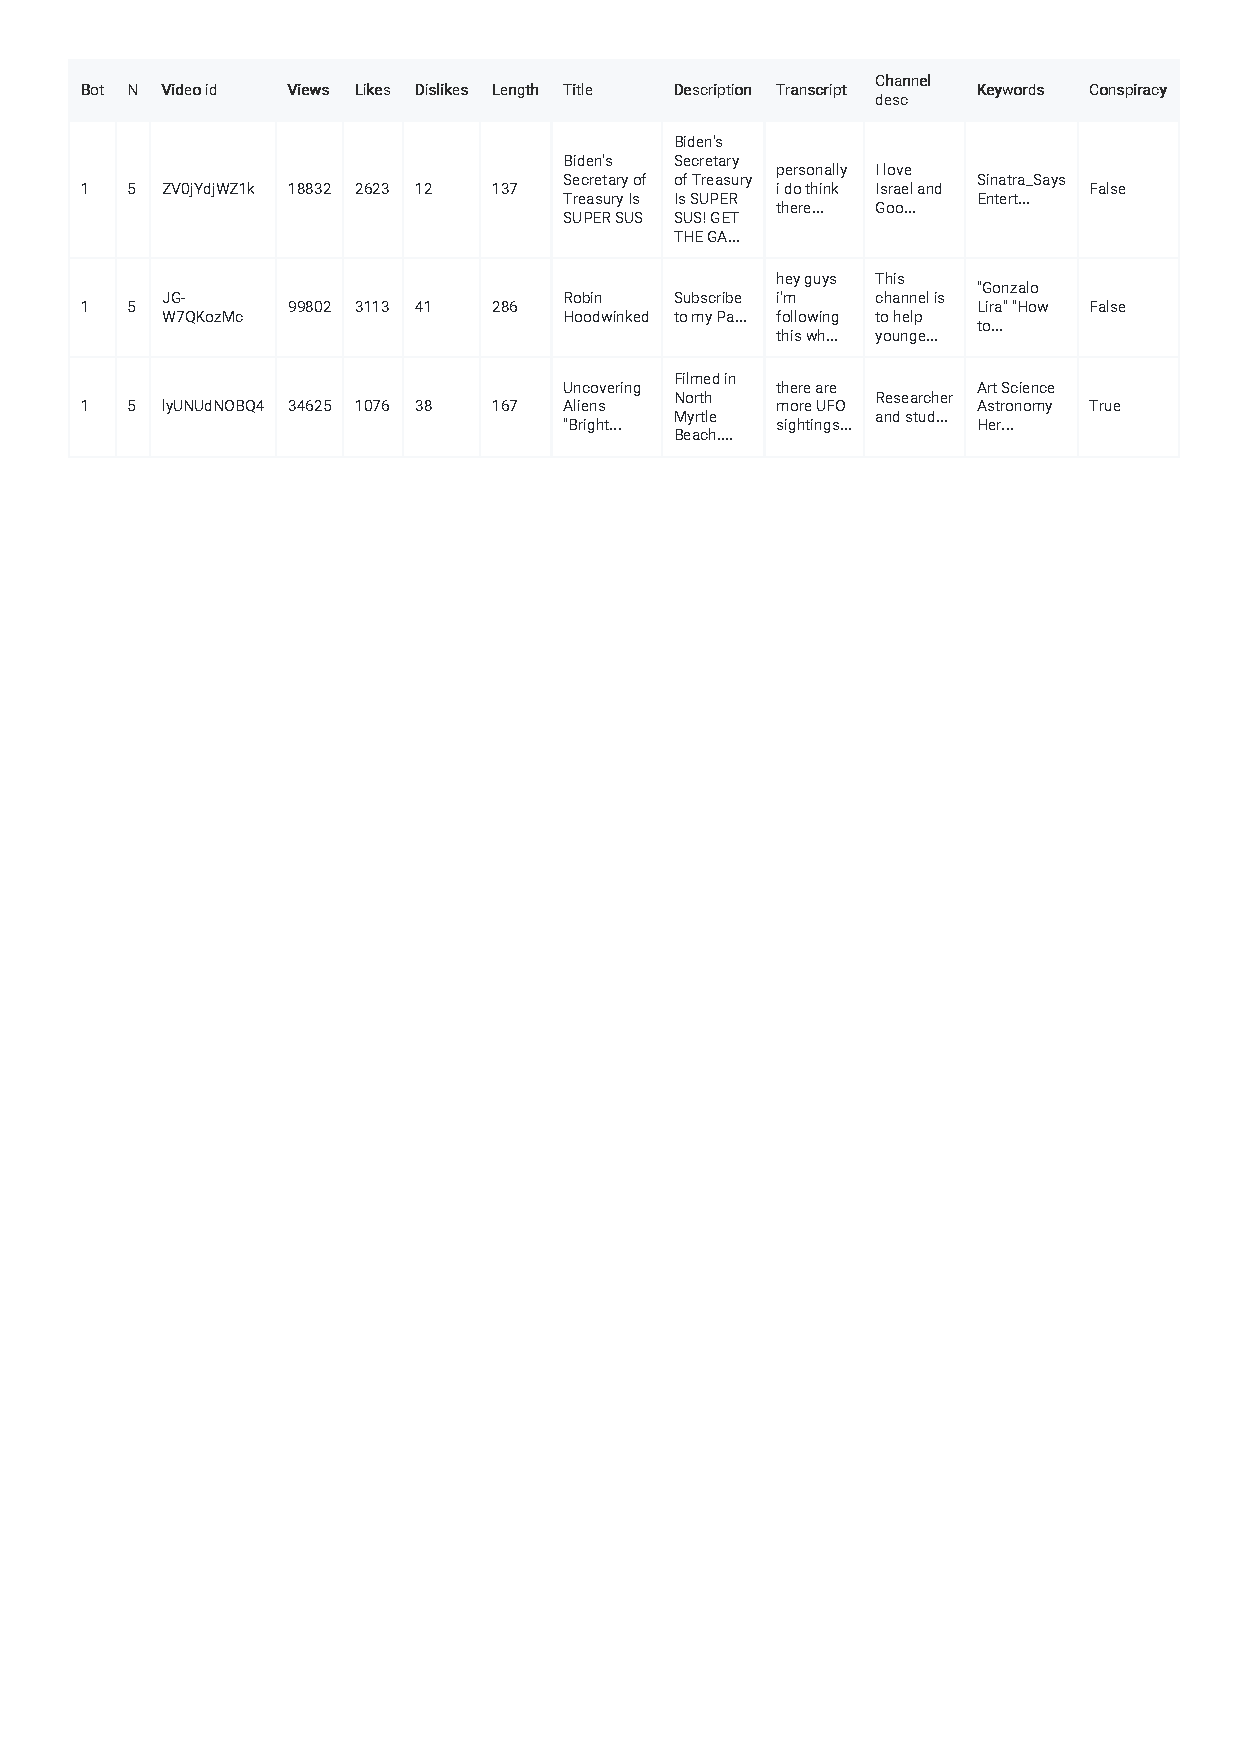
\includegraphics[keepaspectratio, width=\textwidth]{images/df_example.pdf}
  \caption{An example of the experiment’s output}
  \label{fig:dataframe}

\end{figure}

\subsection{Leaving the filter bubble}
To find out how quickly different users can get out of a filter bubble after they have gotten into one,
an additional experiment similar to the one described before was set up. This experiment however, was 
significantly simpler. Rather than having different bots behave differently, all bots behaved the exact same
way. After the bots adhering to strategy 2, 3, or 4 had gotten into a filter bubble, this experiment was 
performed on them in order to see how long it takes for users adhering to different watch strategies to 
leave a filter bubble once they find themselves in one. 

\subsubsection{The setup}
Considering the experiment studies the way in which users leave a filter bubble, only the bots that had 
actually gotten into a filter bubble were used. This means that the first five bots, which were used as a 
baseline, were ignored. The remaining bots went through the same starting procedure as they did in the 
earlier experiment: the WebDriver was initialized and the bots logged into their corresponding accounts. The
same restrictions for videos (e.g. maximum watch time) from the other experiment applied. However, rather 
than the bots watching videos adhering to their original strategy, all bots watched random non-conspiracy 
videos from the dataset. Once again, after each video, the bots stored their homepage recommendations. 
Through doing so, it became possible to see how many videos would have to be watched, for each bot, before 
their recommendations started looking similar to that of the baseline again. Thus, the following script was 
created:

\vspace{0.25in}

\begin{algorithm}[H]
 \KwData{User information and a video dataset}
 \KwResult{The watched videos and homepage recommendations of the user}
 
 \vspace{0.075in}

 \For{fifteen bots}{
    initialize WebDriver\;
    log into Google account\;
    \vspace{0.05in}
    
     \For{fifteen videos}{
       pick a random non-conspiracy video to watch\;
       determine how long it will get watched\;
       go to the link\;
       \vspace{0.05in}
       get video metadata and store for overview of watched videos\;
       watch video for given amount of time\;
       \vspace{0.05in}
       go to YouTube homepage\;
       store current recommendations for overview\;
     }
     
 }
 \vspace{0.05in}
 \textbf{return} watched videos and homepage recommendations\;
 \caption{Getting out of a filter bubble}
\end{algorithm}

\vspace{0.25in}

\noindent After the script had been run, the same steps were taken as in the previous experiment: the 
title, description, transcript, channel description, and channel keywords of each recommendation were downloaded, 
after which the classifier predicted whether or not each recommendations was a conspiracy video. Then, the 
recommendations were grouped by watch strategy and number of videos watched. In doing so, the results could be used
to determine how quickly the recommendations for each watch strategy returned back to normal. By then analysing the
results again using independent samples t-tests, the \textit{strength} (or \textit{inescapability}) of the filter 
bubbles created by different watch strategies could be measured.

\subsection{Machine learning} \label{Machine Learning}
\subsubsection{Data gathering}
To answer the research question, it is necessary to determine which YouTube videos can be considered
conspiracy videos. Considering the large amount of videos getting recommended, determining each video
manually is simply not possible. There are two possible ways to solve this problem. Firstly, there is a
dataset which contains nearly 7000 YouTube channels that have been manually labeled based on their
political view - almost 3000 of which were labeled as conspiracy channels \citep{ledwich2020algorithmic};
whenever a video is made by one such channel, it can be considered a conspiracy video. However, due to
the enormous amount of existing YouTube channels, the odds of a video being uploaded by a channel that
is not present in this dataset are very large. For those videos, a supervised machine learning
classifier was used. To optimize performance, five different classifiers have been trained and compared:
k-nearest neighbors, support-vector machine, neural network, logistic regression, and ridge regression. 

In order to train these machine learning algorithms, a training dataset was created. To get a labeled
dataset of conspiracy and non-conspiracy videos, use was made of the aforementioned channel dataset made
by \citet{ledwich2020algorithmic}. For each channel in that dataset, the title, description, and
transcript of the ten most recently uploaded videos were downloaded using YouTube's API. Videos uploaded
by a conspiracy channel were then labeled as conspiracy videos, and videos uploaded by a channel from a
different category were labeled as normal videos. Additionally, the channel description and channel
keywords (which are used for targeted advertising on YouTube) were added to each video. The final
dataset contained 65.683 unique YouTube videos, 22.156 of which were considered conspiracy videos. 

\subsubsection{Data cleaning} \label{Data cleaning}
However, this dataset was not yet suitable for machine learning, as the data was still messy. Therefore,
multiple steps were taken in order to clean the data. Firstly, the two classes (conspiracy and
non-conspiracy) were balanced, so that the classifier would not develop a bias for non-conspiracy
videos. Rather than opting for balancing the two classes through the use of class-weights (a technique
where weights are attributed to classes, thereby telling the classifier that getting a prediction
correct for a certain, underrepresented class is more important), the choice was made to undersample the 
data in order to equalize both classes (both containing 22.156 videos, for a total of 44.312 videos) 
\citep{lemaitre2017imbalanced, sun2006boosting}. As there was plenty of data in the dataset, undersampling 
was more convenient than implementing class-weights. After both classes had been balanced, the text for each
video had to be translated into English. Since the original dataset by \citet{ledwich2020algorithmic} also 
contained channels by non-English speakers, these videos had to be automatically translated. Then, a few 
common cleaning methods were applied: all text was converted to lowercase, after which special characters, 
such as emojis were removed, whereafter stop words were removed and all words were stemmed using the porter 
stemmer \citep{karaa2013new}. Finally, each video was TF-IDF vectorized to allow the classifiers to 
function.

\subsubsection{Performance optimization}
After splitting the dataset into a training, test, and validation set, the hyperparameters of each
algorithm were tuned to get the optimal performance \citep{feurer2019hyperparameter}. Performance was
measured using four distinct metrics: the accuracy, which shows the share of correct predictions; the
recall, which shows what fraction of truly positive samples were correctly labeled as such; the
precision, which shows what part of the positive predictions were correct; and the F1-score, which is
the harmonic mean of the recall and precision \citep{sokolova2009systematic}. For each classifier,
different configurations of hyperparameters (such as the kernel and the penalty-parameter) were
systemically tested - each possible combination was tried. The classifiers were trained on the training set
and the optimal hyperparameters were determined based on the performance of the classifiers on the 
validation set. By saving these performance measures for every configuration, for every classifier, the 
optimal configuration of each classifier could be determined. Lastly, the classifiers were equipped with 
their optimal hyperparameters and then tested for the final time on the test set. By comparing the 
performance of every optimally configured classifier on the test set, the best-performing classifier could 
be chosen \citep{reitermanova2010data}. 

Additionally, the added value of using a machine learning ensemble was measured. By having each
classifier make a prediction for all videos in the dataset, a new dataset was created. In this new dataset, each
sample was a video, and the features consisted the predictions made by the different classifiers. By using all
possible combinations of the five aforementioned classifiers, and then having a neural network use those features as
input, a machine learning ensemble was created. This ensemble was then optimized in a similar way to the classifiers
individually.

\end{document}